\documentclass[../BachelorAssignment.tex]{subfiles}

\begin{document}
\graphicspath{{\subfix{../Images/}}}


The timeline of the assignment is described in figure \ref{fig:timeline}. In the first week, I will spend time working on different tutorials of MercuryDPM, to get myself familiar with the software. I will also look into the source code of GrainLearning and study the algorithm's structure and mathematics. In the coming weeks (up to and including week 9), different simulations will be carried out as part of the experiment on MercuryDPM, initially using synthesized data with a simplified number of parameters (start with 2: sliding friction and restitution). Two types of experiments will be performed to collect the bulk parameters: Rotating drum and heap test. The corresponding data will then be passed through to assess the ability of GrainLearning in calibrating the sliding friction and restitution. The experimental part of the report will start as soon as positive experimental results are obtained, projected to be after week 4, and I will start writing about the technologies used, background knowledge, and simulation procedure while I am researching it. During the assignment, I will be keeping a journal and agendas of all meetings to document the process. Progress meetings are scheduled in week 5 and 8, respectively, to dicsuss the direction of the project.

\begin{figure}[H]
    \centering
    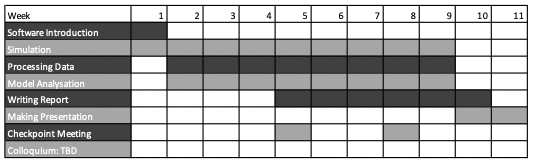
\includegraphics[scale=0.8]{timeline.png}
    \caption{Timeline of the Assignment}
    \label{fig:timeline}
\end{figure}



\end{document}